\documentclass[10pt,twocolumn,letterpaper]{article}

\usepackage{dependable_dnn}
\usepackage{times}
\usepackage{epsfig}
\usepackage{graphicx}
\usepackage{amsmath}
\usepackage{amssymb}
\usepackage{subfigure}
\usepackage[table, dvipsnames]{xcolor}

% Include other packages here, before hyperref.

% If you comment hyperref and then uncomment it, you should delete
% egpaper.aux before re-running latex.  (Or just hit 'q' on the first latex
% run, let it finish, and you should be clear).
\usepackage[pagebackref=true,breaklinks=true,letterpaper=true,colorlinks,bookmarks=false]{hyperref}

\iccvfinalcopy % *** Uncomment this line for the final submission

\def\iccvPaperID{} % *** Enter the Paper ID here
\def\httilde{\mbox{\tt\raisebox{-.5ex}{\symbol{126}}}}

% Pages are numbered in submission mode, and unnumbered in camera-ready
\ificcvfinal\pagestyle{empty}\fi
\newcommand{\N}{{\mathbf{N}}}  
\newcommand{\R}{{\mathbf{R}}}  
\newcommand{\A}{{\mathbf{W}}}   
\newcommand{\n}{{\mathbf{n}}}   
\newcommand{\argmax}{\mathop{\arg\max}}  % notation of argmax.

\begin{document}

%%%%%%%%% TITLE - PLEASE UPDATE
\title{Learning to Optimize Domain Specific Normalization for Domain Generalization\\ {\rm {\normalsize Seungmin Lee (profile2697@gmail.com; 2020-20866), \\Dept. of Electrical and Computer Engineering, Seoul National University}}}   % **** Enter the paper title and student information here

\maketitle
\thispagestyle{empty}

\section{Introduction}
This work proposes a multi-source domain generalization method that uses various normalization layers while training separate affine parameters for each domain. The proposed method shows better performance than previous domain generalization methods.


\section{Method}
The proposed method holds a domain-specific normalization (DSON) layer for each domain. The proposed normalization layer consists of a pair of the batch norm and instance norm layers, while DSON's mean and variance are the weighted sum of the corresponding statistics from the batch norm and instance norm. Note that each DSON layer possesses its affine parameters. 
In training, the proposed method normalizes activations using the corresponding DSON layer, and it updates each set of affine parameters in the normalization layers. At inference, the proposed method transforms activations using all DSON layers and averages them. 

\section{Results}
The authors conduct experiments on various domain generalization benchmarks to verify the effectiveness of the proposed method. DSON shows consistent performance improvements across all the benchmarks.
An interesting results is shown in Fig.~\ref{fig:imgs2}. As we can observe, the ratio of instance norm is higher in the multi-source experiments. The result supports that instance normalization is beneficial to alleviate domain shifts.

\begin{figure}[h]
	\centering
	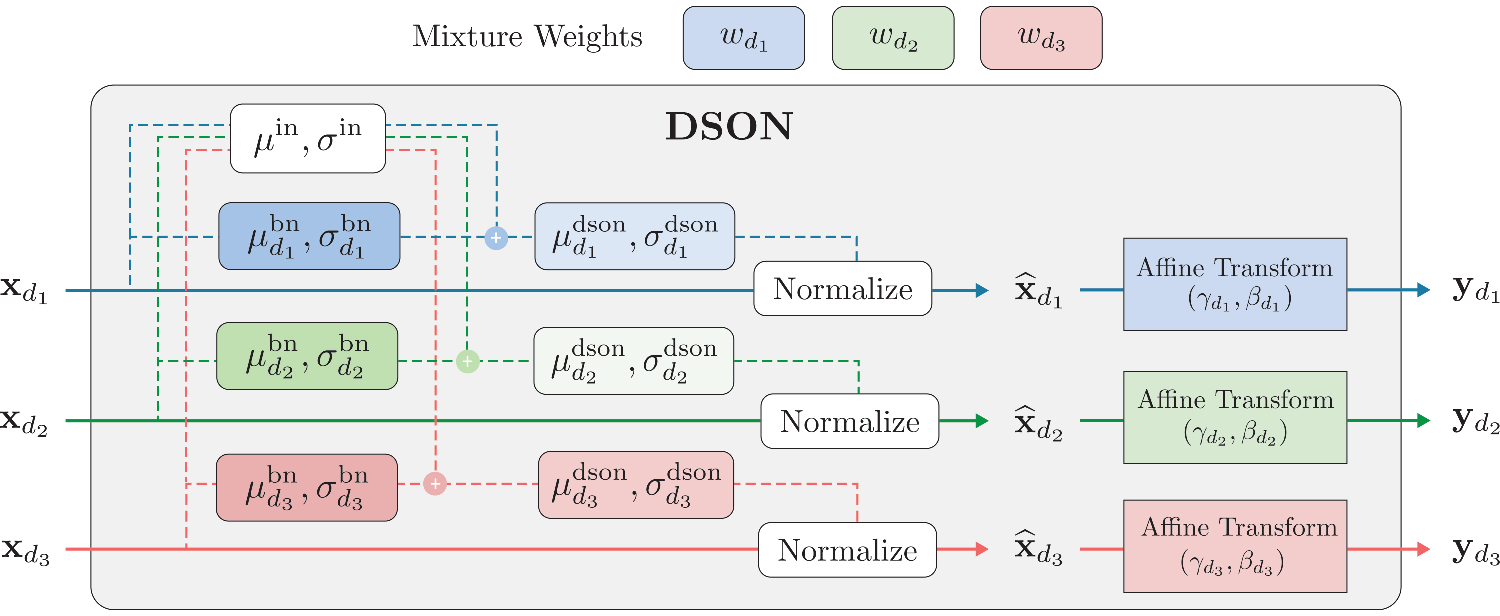
\includegraphics[width=8cm]{assets/DSON.pdf}
	\caption{The architecture of DSON.}
	\label{fig:imgs}
\end{figure}

\begin{figure}[t]
	\centering
	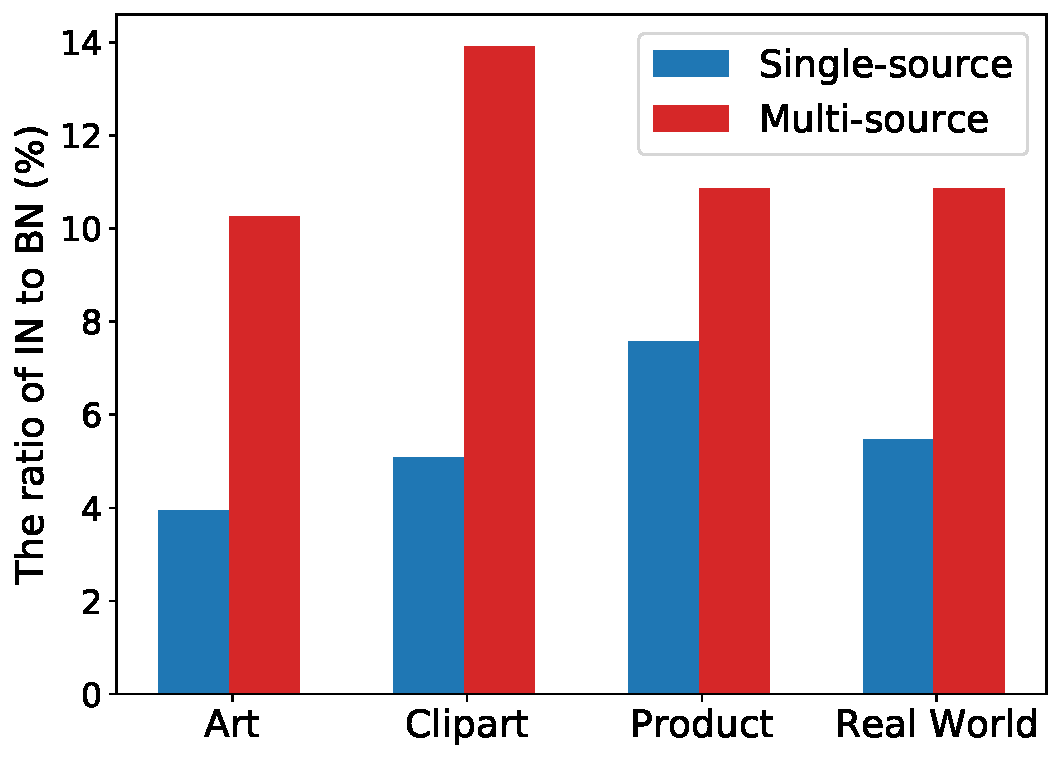
\includegraphics[width=8cm]{assets/in_office.pdf}
	\caption{The ratio of instance norm increases in multi-source experiments.}
	\label{fig:imgs2}
\end{figure}

\section{Personal Note}
The proposed method is simple and effective. However, DSON requires more computations at inference time, limiting the method's usefulness. Moreover, DSON seems to have a limited novelty.

\end{document}
